
\thispagestyle{empty}

\vspace*{5em}


\centerline{\includegraphics[scale=1.0,clip]{figures/by-sa.eps}}
Djelo \emph{Grupe, simetrije i tenzori u fizici}, čiji je autor Krešimir
Kumerički, ustupljeno je pod licencom Creative Commons 
"Imenovanje-Dijeli pod istim uvjetima" (\emph{Attribution-ShareAlike}) 
4.0 nelokalizirana licenca. Za uvid u tu licencu, posjetite
\url{http://creativecommons.org/licenses/by-sa/4.0/}.

Izvedenice ove knjige (npr. izolirani dijelovi ili modificirane verzije knjige) moraju minimalno
navesti 1. izvornog autora 2. izvorni naziv knjige 3. modifikacije, ako ih ima i
4. poveznicu na GitHub repozitorij
\url{https://github.com/kkumer/simetrije} putem kojeg je ova knjiga
slobodno dostupna.

\vspace*{3em}
Slika na naslovnici: Niles Johnson, \emph{Hopfova fibracija}\\
TikZ k\^{o}d ilustracija u knjizi: Mark Anthony Bromuela, Sveučilište Chittagong

\vspace*{3em}
\textcopyright{} 2025. Krešimir Kumerički. Sva prava pridržana.\\
\small
Dokument odgovara \texttt{git} verziji \texttt{\githash} (tag: \texttt{\gittag}) datuma \gitdate.

\cleardoublepage
\thispagestyle{empty}
\vspace*{10em}
\begin{flushright}
    \emph{Mojim roditeljima}
\end{flushright}
\cleardoublepage
